\documentclass[a4paper]{article}

\usepackage[utf8]{inputenc}
\usepackage[T1]{fontenc}
\usepackage{graphicx}
\usepackage{float}
\usepackage{caption}

\begin{document}
\section*{Hanghuhn}
\begin{figure}[H]
\centering
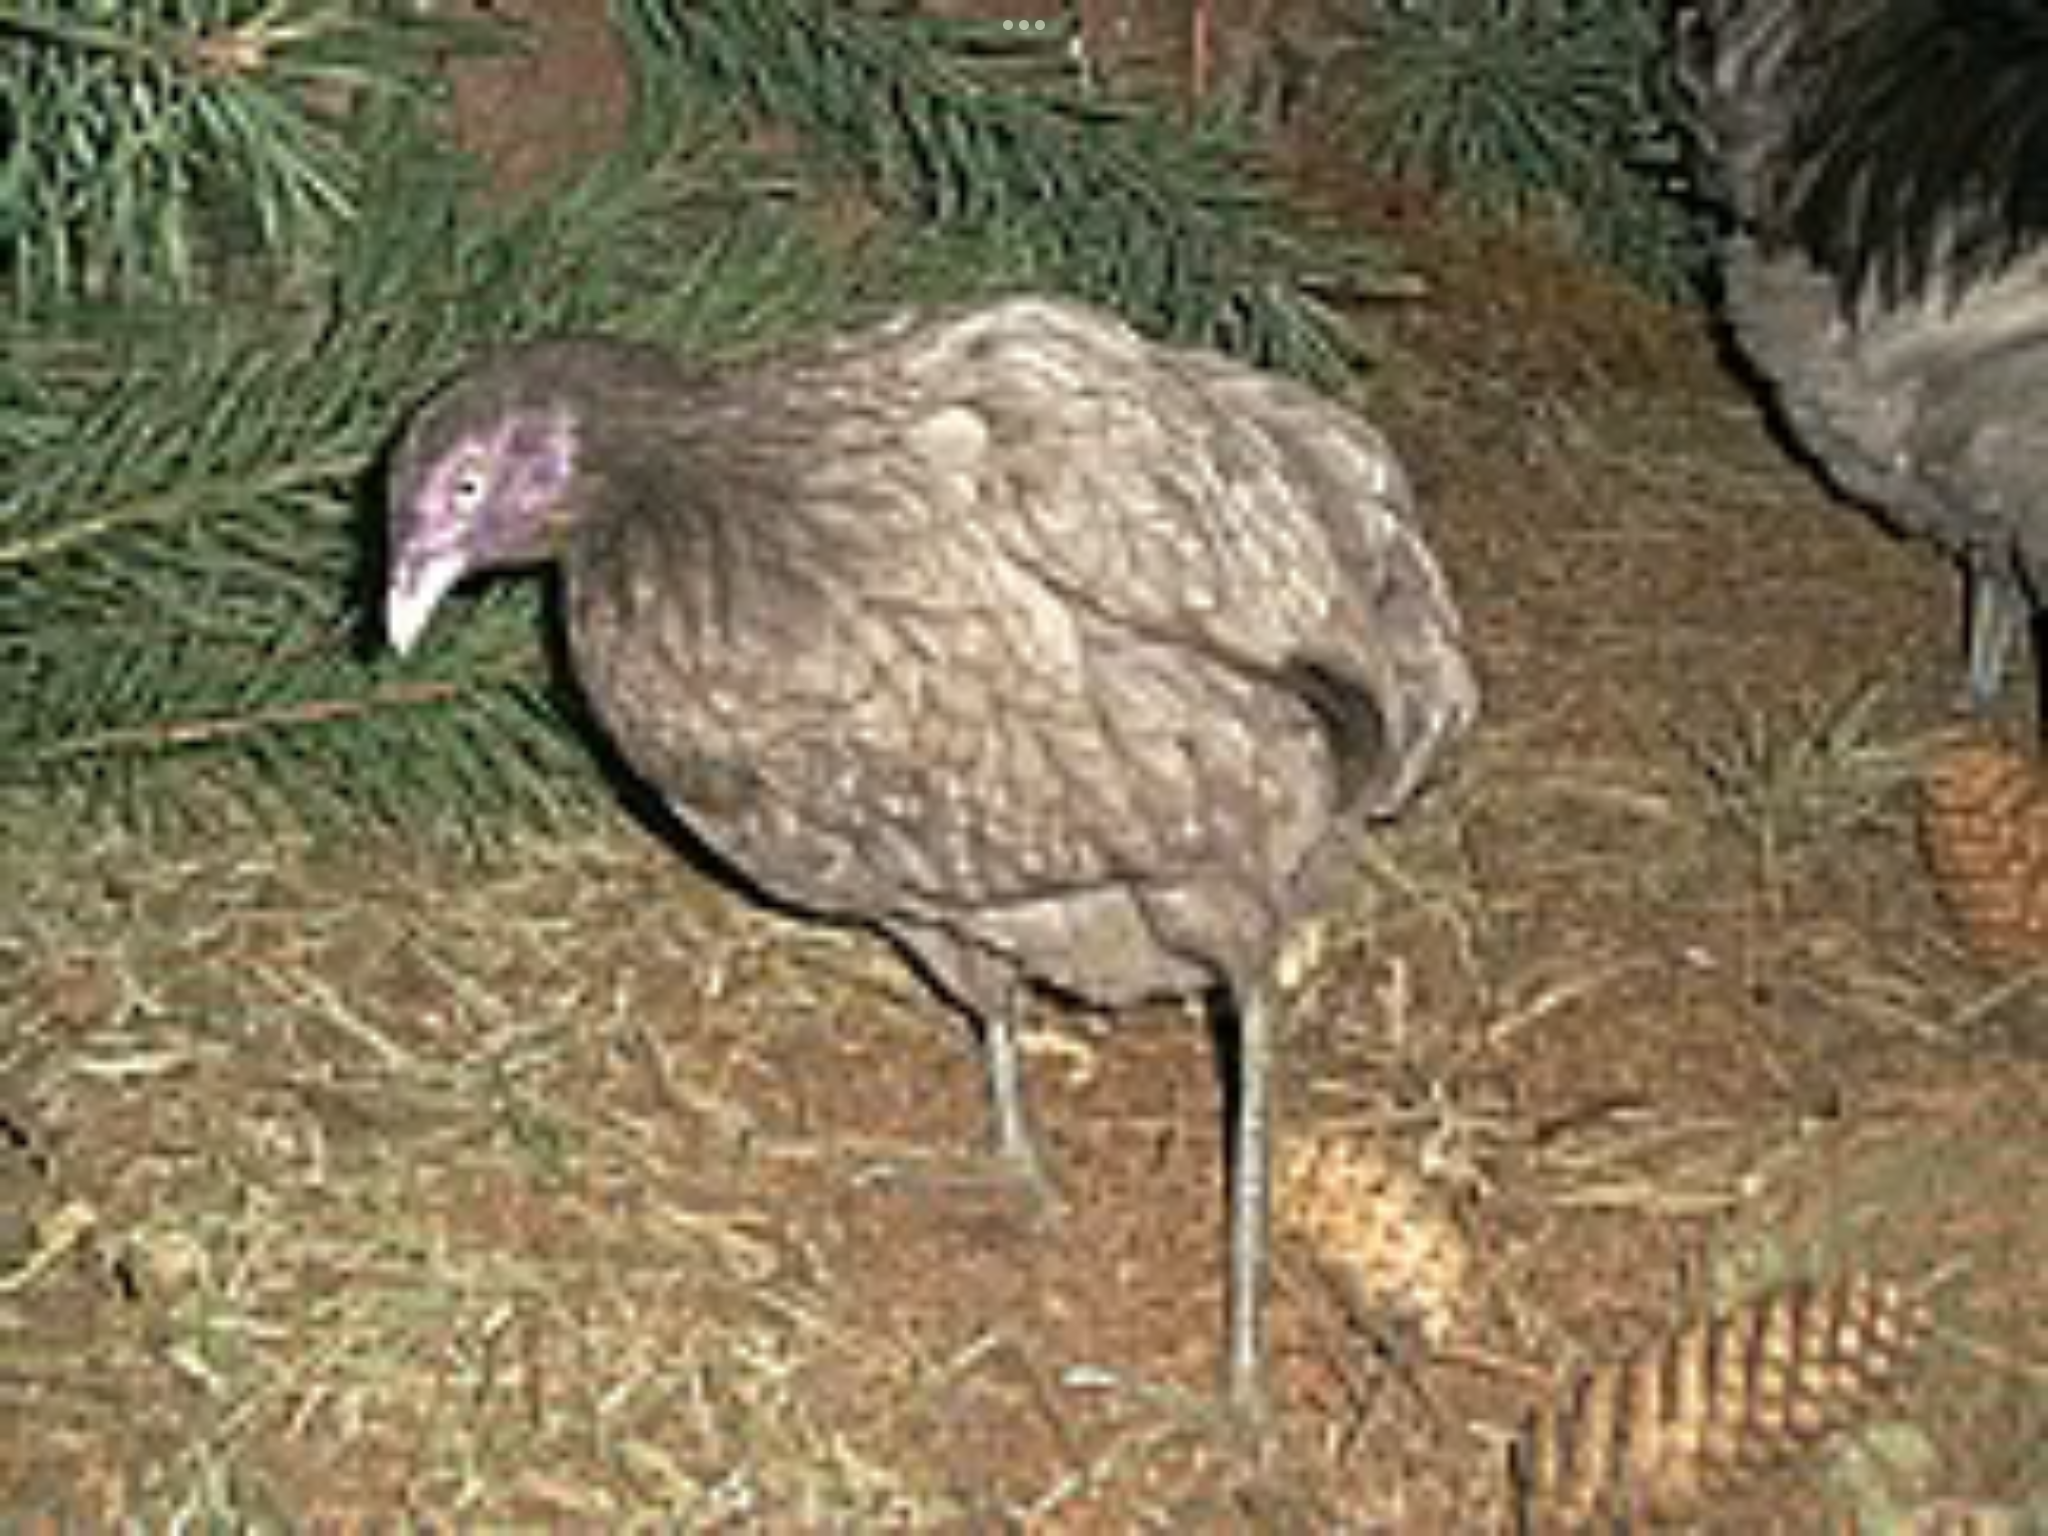
\includegraphics[height=0.3\textheight]{Hanghuhn.PNG}
\caption*{Hanghuhn in seinem natürlichen Lebensraum}
\label{fig:hanghuhn}
\end{figure}
Das gemeine Hanghuhn (gallus gallus conatus) ist ein Huhn mit zwei verschieden
langen Beinen. Es hat diese durch evolutionäre Anpassung an seinen natürlichen
Lebensraum, den Hang oder Deich entwickelt, um auf schrägem Untergrund besser
stehen zu können. Die Hanghühner gliedern sich in
zwei Unterarten: Das rechte Hanghuhn (gallus gallus conatus dextra) und das
linke Hanghuhn (gallus gallus conates sinistra). Bei rechten Hanghuhn ist das
rechte Bein und der rechte Flügel jeweils länger bzw. größer als das linke
Bein und der linke Flügel, beim linken Hanghuhn ist dies genau umgekehrt.
Augrund eben jener Physis ist das Hanghuhn im Flug ausschließlich in der Lage,
eine orbikuläre Bahn zu beschreiben. Ein männliches Hanghuhn heißt Hanghahn
oder Hanggockel. Wenn ein Hanghuhn sich umdreht, fällt es zwangsläufig den
Hang hinunter. Der Hanggockel muss daher, falls er sich auf dem Hang vor der
Hanghenne befindet, zur Paarung eine Weile rückwärts laufen. Hanggockel, die
dabei scheitern, disqualifizieren sich als Partner. Kreuzungen zwischen linken
und rechten Hanghühnern gestalten sich durch die Anpassung der Hühner an ihren
jeweiligen Hang als besonders schwierig und sind in freier Wildbahn nahezu
ausgeschlossen.\\
Hanghühner bauen ihre Nester schräg an den Hang und müssen dabei besonders
darauf achten, dass die Eier nicht aus dem Nest und anschließend den Hang
hinunterrollen, sonst schlüpfen aus ihnen ganz gewühnliche Haushühner.
Aufgrund dieser Tatsache ist das Hanghuhn in weiten Teilen der Welt vom
Aussterben bedroht und aktuell ist dem Verein der Freunde des linken Hanghuhns
e.v. keine Population in Therman mehr bekannt. Vereinspräsident Gabriel von
Hohenhahnheim unternahm allerdings unlängst eine beschwerliche Reise in den
gebirgigen Norden von Walkorst, und fand dort zu seiner großen Freude eine
intakte Hanghuhnpopulation. Aus seinen Forschungstagebüchern geht hervor, dass
die dortigen Hühner Eier mit einer abgeplatteten Seite legen, die weniger
leicht aus dem Nest rollen.
\end{document}
